\documentclass[border=6pt]{standalone}
% Shared TikZ styles for the network diagrams.
\usepackage{tikz}
\usetikzlibrary{arrows.meta,positioning}
\definecolor{nodeblue}{HTML}{2A78D6}
\definecolor{endfill}{HTML}{E3EEFB}
\definecolor{shortcut}{HTML}{D64545}
\tikzset{
  v/.style={circle, draw=nodeblue, line width=1pt, minimum size=9mm, inner sep=0pt, font=\small},
  od/.style={v, fill=endfill},
  e/.style={-{Latex[length=2.6mm]}, line width=0.8pt},
  free/.style={e, shortcut},
  c/.style={font=\footnotesize, fill=white, inner sep=1.5pt},
}

\begin{document}
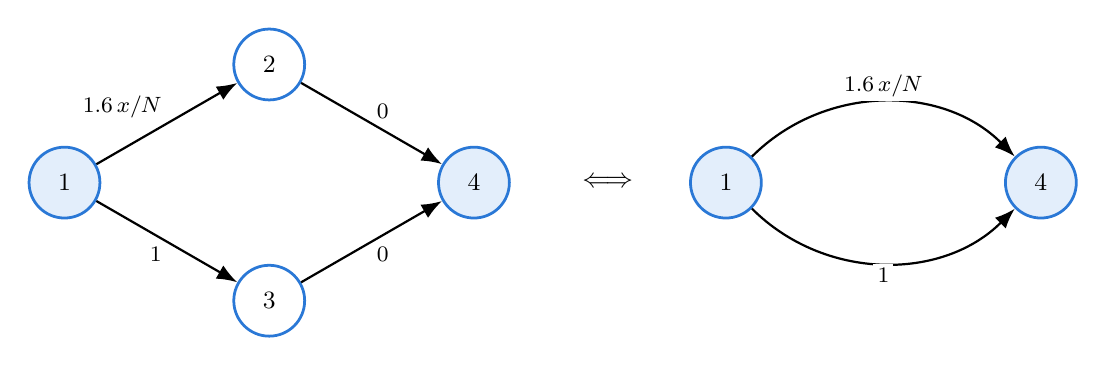
\begin{tikzpicture}
  \node[od] (1) at (0,0) {1};
  \node[v]  (2) at (2.6,1.5) {2};
  \node[v]  (3) at (2.6,-1.5) {3};
  \node[od] (4) at (5.2,0) {4};
  \draw[e] (1) -- node[c, above left] {$1.6\,x/N$} (2);
  \draw[e] (1) -- node[c, below left] {$1$} (3);
  \draw[e] (2) -- node[c, above right] {$0$} (4);
  \draw[e] (3) -- node[c, below right] {$0$} (4);

  \node at (6.9,0) {$\Longleftrightarrow$};

  \node[od] (a) at (8.4,0) {1};
  \node[od] (b) at (12.4,0) {4};
  \draw[e] (a) to[bend left=45]  node[c, above] {$1.6\,x/N$} (b);
  \draw[e] (a) to[bend right=45] node[c, below] {$1$} (b);
\end{tikzpicture}
\end{document}
